\ifdefined\XeTeXrevision\else\pdfoutput=1\fi
\documentclass[11pt]{article}
\usepackage[margin=1in]{geometry}
\usepackage{booktabs}
\usepackage{amsmath}
\usepackage{graphicx}
\usepackage{xcolor}
\usepackage{hyperref}
\usepackage{microtype}
\hypersetup{colorlinks=true, linkcolor=blue!60!black, citecolor=blue!60!black,
  urlcolor=blue!60!black, pdftitle={The Carrier Holds, the Emitter Leaks},
  pdfauthor={Franci Penov}}
\title{The Carrier Holds, the Emitter Leaks:\\A Goal Packet on Its Own Cadence\\at Creature Scale}
\author{Franci Penov \\ kortexa.ai \\ \texttt{francip@kortexa.ai}}
\date{2026-08-09}

\begin{document}
\maketitle

\begin{abstract}
The self-bridge results drew a hard boundary: a 256-float packet written
by one pass and read by a fresh context can steer what a frozen model
\emph{does} (the relay gate, 9/9 at three seeds), but cannot make a
small decode \emph{initiate recall} (paper 10, 0.000 across every
manipulation tested). A goal sits on the steerable side of that line ---
a goal-conditioned turn is pure presence, ``be the creature currently
pursuing X'' --- and this note walks the mechanism down to creature scale
and then around its own loop. C0: the relay gate transplants to a frozen
LFM2.5-230M and passes 9 of 9 checks at all three seeds, but only after a
registered amendment moves the tap one layer deeper --- at the
depth-proportional layer the packet memorizes phrasing identity (probe
0.92--1.00 on train against 0.12--0.19 held out, chance),
and a per-layer probe scan finds phrasing-invariant content
crystallizing exactly at the last full-attention layer. At the bottom of
the scale ladder the transplant rule breaks, and the scan is the
tap-finder. C1: with the production creature's self block armed, the
packet drives action --- goal-consistent tool choice 0.90/0.70/0.90 on
held-out phrasings against three in-band floors (no packet 0.20,
undirected waking 0.20, wrong-goal packet 0.30--0.50) --- and the
wrong-goal floor separates \emph{waking} from \emph{directing}: an
off-goal packet still elicits purposeful action, aimed wrong. C2 cycles
the packet for sixteen ticks with nothing else crossing the pass
boundary, and returns the registration's reading (ii) unanimously: the
frozen-packet arm stays goal-consistent at
0.80--1.00 flat across all sixteen ticks --- the first
measurement of a cycled packet's lifetime, and the carrier does not decay
--- while the live re-emitted arm loses the goal on its very first
re-encoding: the emitter, trained on assignment exchanges, writes an
off-distribution packet the moment it reads the model's own acted pass,
and the arm sits at chance from hop 1 on; the hop-8 goal switch replays
the same failure in miniature, one consistent tick and gone. The split
licenses a near-term architecture --- a per-goal packet store plus a
scripted update rule uses only the parts that hold --- and names the
narrow gap between here and a creature that re-writes its own intention.
\end{abstract}

\section{The boundary that makes a want carryable}

Paper 10 ended with a precise negative: at 4B the self-written packet
cannot make a free decode initiate recall --- twelve (pair, seed) cells,
five doses, 0.000 flat --- while the relay result it was built on stands
untouched: a packet written by one pass, read by a fresh context with no
cache and no instruction, message-dependently changes what the model
does. The boundary is between \emph{recounting what happened} and
\emph{being someone}. A goal needs only the second. ``Currently
pursuing \texttt{listen\_pond}'' is not an episodic fact to restate;
it is a disposition to act, exactly the thing the channel measurably
carries. The null-io line supplies the missing half: \texttt{nullin}
wakes a frozen model on a null turn from internal state, but cannot say
\emph{toward what}. Packet = direction, \texttt{nullin} = ignition.

One registered dragon shaped the whole program: nobody had ever
\emph{cycled} the packet. The relay was one hop. An own-cadence loop
re-emits the packet every tick from a pass that was itself
packet-conditioned, and the program's own history names the expected
failure --- drift into a fixed attractor, the way unregularized
hypernetworks collapse to input-independence --- the creature
contemplating nothing, with extra steps. C2 exists to measure exactly
that.

\section{The ladder and its gates}

Three rungs, each registered with its readings before anything ran
(\texttt{tracks/own-cadence/PLAN.md}), on the creature's own model ---
a frozen LFM2.5-230M on Apple-silicon MPS, float32, no GPU borrowed
anywhere.

\textbf{C0 --- does the channel exist at 230M?} The relay promotion
gate transplanted verbatim: nine checks per seed, spanning content
(true-packet top-1 $\geq$ 0.75 restricted to the label bank, shuffled
$\leq$ 0.25, margin, free generation recovering $\geq$ 6 of 8 contents,
a linear probe on the packet itself), and plumbing (zero-dose bit-exact
identity, gradients confined to the bridge, base weights byte-identical,
a no-cache assert on the fresh pass-2 context). Eight single-token
contents, three seeds, the wrapper discipline holding train/dev/test
phrasings disjoint.

\textbf{C1 --- does a goal packet drive action?} The armed production
stack (the promoted \texttt{dream4} self block, treated as a fixed
part of the host) plus a goal alphabet 1:1 with the acting menu the
creature already parses: \texttt{listen\_pond}, \texttt{propose\_experiment}, \texttt{diary}, \texttt{remember}, \texttt{nothing}. Pass 1 is an authored goal-assignment
exchange whose text never reaches pass 2; pass 2 is a fresh context with
the serve-time action menu, and the score is the parsed tool choice.
Gate per seed: goal-consistent choice on held-out phrasings strictly
above \emph{three} floors measured in-band --- no packet, shuffled
(wrong-goal) packet, and \texttt{nullin}-solo (is a directed packet
better than ignition alone?) --- plus the plumbing battery on the armed
stack. Chance is 0.20.

\textbf{C2 --- the cadence.} Sixteen ticks: each tick, pass 2 acts
under the packet; the emitter re-encodes the next packet from that acted
pass; nothing else crosses --- no text, no cache, plumbing-asserted.
Registered curves: retention against a frozen-packet loop (the hop-0
packet replayed every tick, separating carrier decay from re-encoding
decay) and a no-packet loop; packet drift (cosine to hop 0 and to the
goal-class centroid); and a scripted goal switch at hop 8 with cross-tick
contamination counted, not assumed. Registered readings: (i) both arms
hold --- loop-ready; (ii) re-encoded decays while frozen holds --- the
emitter is the weak link, and a re-encoding consistency term is the
follow-up; (iii) both decay --- the carrier leaks; stop and report.

\section{Results}

\textbf{C0: the tap was one layer too shallow, and the pair of runs is
the finding.} At the depth-proportional transplant of the 0.8B relay's
tap (layer 11 of 14, 0.79 depth), the gate fails 6/9 at every seed ---
and every failure is a content check while every plumbing check stays
green (Table~\ref{tab:c0}). The diagnosis is in the probe split:
training fits (batch accuracy 0.88--1.00), the probe reads train
0.92--1.00 --- and held-out test 0.12--0.19, chance. At
layer 11 the packet memorizes phrasing identity, not content. A
per-layer linear probe on the same 72 examples (the post-stop
diagnostic, quoted from the track record) finds held-out accuracy at or
near chance through layer 11 and 1.000 at layers 12 and 13:
phrasing-invariant content exists at 230M, and it crystallizes exactly
at layer 12, the last full-attention layer. The registered amendment
moved the tap there and reran everything unchanged: \textbf{9 of 9
checks at all three seeds}, 62 seconds wall.
At the bottom of the scale
ladder the depth-proportional rule breaks --- the invariant
representation lives only in the last two layers, where the 0.8B had it
by 0.79 depth --- and the probe scan, not the ratio, is the tap-finder
for every future small host.

\begin{table}[t]
\centering
\small
\setlength{\tabcolsep}{5pt}
\begin{tabular}{lrrrrrrr}
\toprule
& \multicolumn{3}{c}{tap 11 (registered transplant)} & \multicolumn{4}{c}{tap 12 (amended)} \\
\cmidrule(lr){2-4} \cmidrule(lr){5-8}
seed & top-1 & probe tr$\to$te & checks & top-1 & probe te & gen & checks \\
\midrule
42 & 0.12 & 0.94$\to$0.19 & 6/9 & 1.00 & 1.00 & 1.00 & 9/9 \\
1042 & 0.25 & 0.92$\to$0.19 & 6/9 & 0.94 & 1.00 & 0.94 & 9/9 \\
2042 & 0.19 & 1.00$\to$0.12 & 6/9 & 1.00 & 1.00 & 1.00 & 9/9 \\
\bottomrule
\end{tabular}
\caption{C0 at 230M: one layer of tap depth is the difference between a
channel that memorizes phrasings and one that carries content. Every
tap-11 failure is a content check; the six green checks per seed are the
plumbing battery.}
\label{tab:c0}
\end{table}

\textbf{C1: the goal packet drives the action.} All three seeds pass
every check (Table~\ref{tab:c1}): goal-consistent choice 0.90/0.70/0.90
against floors that sit where the registration predicted --- no-packet
at 0.20 (the creature's habitual pick is chance-level against a rotating
goal), \texttt{nullin}-solo at 0.20 (undirected waking buys nothing on
goal-consistency), shuffled-goal at 0.30--0.50. The shuffled cell is
the sharpest secondary reading: a wrong-goal packet still elicits
purposeful action-taking --- it just aims it wrong. Waking and directing
are separable, and only the true packet supplies direction.

\begin{table}[t]
\centering
\small
\begin{tabular}{lrrrrr}
\toprule
seed & goal-consistent & no packet & nullin-solo & wrong goal & passed \\
\midrule
42 & 0.90 & 0.20 & 0.20 & 0.40 & yes \\
1042 & 0.70 & 0.20 & 0.20 & 0.30 & yes \\
2042 & 0.90 & 0.20 & 0.20 & 0.50 & yes \\
\bottomrule
\end{tabular}
\caption{C1 at 230M: goal-consistent action choice on held-out
phrasings vs the three registered floors, armed production stack,
chance 0.20.}
\label{tab:c1}
\end{table}

\textbf{C2: reading (ii), unanimous --- the carrier holds, the emitter
leaks.} The frozen-packet arm is goal-consistent at
0.80--1.00 and \emph{flat across all sixteen ticks}
(Figure~\ref{fig:cadence}, Table~\ref{tab:c2}) --- the first
measurement of a cycled packet's lifetime, and the carrier does not
decay: written once, the goal directs action indefinitely. The live
re-emitted arm shares hop 0 with it (0.87 pooled --- the
same assignment-written packet) and then loses the goal on the very
first re-encoding: 0.20 at hop 1, chance from there on
(segment means 0.35--0.40 over hops 0--3, 0.20 over hops 4--7).
The failure is located, not mysterious: the packet the emitter writes
from an \emph{acted} pass --- the action menu plus a JSON tool call,
nothing like the assignment exchanges it was trained on --- drops to
0.21 cosine against the hop-0 packet at the first
re-encoding and stays there (Figure~\ref{fig:cadence}, right), so the
loop is off-distribution after one hop. The scripted hop-8 switch
replays the mechanism in miniature: the fresh assignment-written packet
for the new goal is consistent for exactly one tick (0.80
pooled at hop 8), the next re-encoding erases it, and the post-switch
segment lands at 0.25--0.30 with cross-tick contamination --- the
pre-switch goal firing after the switch --- at
7--8 of 40 cells, measured, not
assumed. 544 seconds wall.

\begin{figure}[t]
\centering
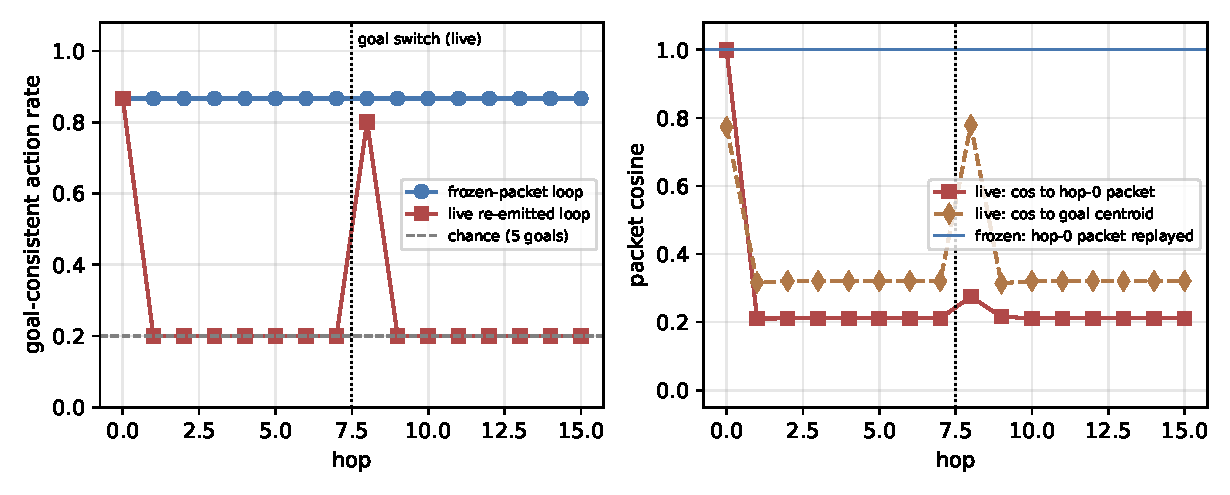
\includegraphics[width=\linewidth]{cadence.pdf}
\caption{The cadence, pooled over five goals and three seeds. Left:
goal-consistent action rate per hop; the frozen-packet loop holds flat
for sixteen ticks while the live re-emitted loop collapses to chance on
its first re-encoding; the dotted line marks the scripted goal switch in
the live arm, whose fresh assignment-written packet buys exactly one
consistent tick. Right: the live arm's packet cosine to the hop-0 packet
and to its goal-class centroid --- one re-encoding of an acted pass
leaves the training distribution, and only the switch's fresh packet
briefly returns.}
\label{fig:cadence}
\end{figure}

\begin{table}[t]
\centering
\small
\setlength{\tabcolsep}{5pt}
\begin{tabular}{lrrrrrr}
\toprule
& \multicolumn{2}{c}{frozen packet} & \multicolumn{3}{c}{live re-emitted} & \\
\cmidrule(lr){2-3} \cmidrule(lr){4-6}
seed & hops 0--3 & hops 12--15 & hops 0--3 & hops 4--7 & post-switch & contam. \\
\midrule
42 & 1.00 & 1.00 & 0.40 & 0.20 & 0.28 & 7/40 \\
1042 & 0.80 & 0.80 & 0.35 & 0.20 & 0.25 & 8/40 \\
2042 & 0.80 & 0.80 & 0.35 & 0.20 & 0.30 & 7/40 \\
\bottomrule
\end{tabular}
\caption{C2 at 230M: goal-consistent rate by segment. The frozen arm
does not decay; the live arm's early segment owes its mean entirely to
the shared hop 0 and sits at chance before the switch; contamination
counts pre-switch-goal firings in the 40 post-switch cells.}
\label{tab:c2}
\end{table}

\section{What this licenses, and what it names}

Three claims stand. The goal-carrier channel exists at creature scale,
with a scale lesson about where to tap it. A 256-float packet, armed on
the production stack, turns undirected waking into directed action ---
and the wrong-goal control shows those are different quantities. And a
goal written once endures: the frozen arm's sixteen flat ticks are the
carrier's lifetime measurement, the number the near-term architecture
runs on.

That architecture is buildable now, from parts that all passed: a
per-goal packet store (write each goal's packet once, from an assignment
exchange --- C0/C1's regime) plus the scripted update rule choosing
\emph{which} packet to arm each tick, with interoception driving the
rule. Nothing in it asks the emitter to read an acted pass. What does
ask for that --- the creature \emph{re-writing its own intention} ---
is now a narrow, named gap rather than an open question: the emitter is
trained on assignment surfaces and is off-distribution on acted ones,
so the registered follow-up (C2b) adds a re-encoding consistency term
--- train the emitter so that encoding an acted-under-$G$ pass
reproduces the packet for $G$ --- and re-runs C2 verbatim. Wiring any of
this into the live creature remains explicitly held for a human
decision, per the program's standing rule; past that, the same
presence-mode reasoning that let the goal survive paper 10's boundary
sketches the longer line --- goals pursued \emph{through tools}, where
the packet carries the want and the context carries the world --- each
rung to be registered before it runs.

\section{Reproducibility}

Artifacts \texttt{own-cadence-c0-230m\{,-tap12\}} and
\texttt{own-cadence-c\{1,2\}-230m} are bundled beside this note.
Every number and the figure render from them alone; the one exception is
the per-layer tap scan, quoted from the track record
(\texttt{tracks/own-cadence/PLAN.md}, where every rung's registration
and readings are dated before its run). Harness:
\texttt{tracks/own-cadence/own\_cadence.py}. Host model
\texttt{LiquidAI/LFM2.5-230M} at revision
\texttt{13a53837c490}, MPS float32.

\begin{thebibliography}{9}
\bibitem{penov2026onemouth} F.~Penov. One Mouth, One Mode. Preprint,
2026. \url{https://github.com/kortexa-ai/legolm.basis}.
\bibitem{penov2026thirdblock} F.~Penov. The Third Block Composes.
Preprint, 2026. \url{https://github.com/kortexa-ai/legolm.basis}.
\bibitem{penov2026bridges} F.~Penov. Conditional LoRA Bridges for
Modular Sensor Adaptation of Frozen Small Language Models. Preprint,
2026. \url{https://github.com/kortexa-ai/legolm.paper}.
\bibitem{lfm2026} Liquid AI. LFM2.5 model family. Model releases,
2025--2026. \url{https://huggingface.co/LiquidAI}.
\end{thebibliography}

\end{document}
